\section{Background \& Motivation}

\subsection{Functions as a Service}

In FaaS, application developers can create small functions that are triggered by specific events (such as HTTP requests, message queue events, cloud notifications, etc.). 
The entire execution and management of the user-defined functions is managed by the FaaS provider, such as AWS Lambda, Azure Functions, Google Cloud Functions, etc.
This high level of abstraction is distinct from the more conventional cloud abstractions like virtual servers, since users don't have to be concerned with explicit resource allocation.
Instead, functions are automatically invoked in response to their associated events, and the FaaS provider takes care of their entire execution lifecycle.
FaaS tends to have very fine-grained pricing, and function invocations are often charged by milliseconds of CPU time.

This true pay-per-use pricing model, the relative ease of distributed application development, and seamless elastic scaling has led to FaaS as a popular way to develop and deploy distributed and cloud applications.
A wide range of applications such as web services, API services, machine learning inference, IoT backends, and even scientific computing are being deployed as a collection of functions.
FaaS has thus truly emerged as a common abstraction and interface for accessing and harnessing cloud resources.  
FaaS can also be provided on local computing clusters by using frameworks like OpenWhisk, OpenFaaS, etc. 

% Programming model
While FaaS has been a boon for applications, its programming model has many unique execution characteristics that impose new performance tradeoffs, which has motivated new techniques in systems research. 
Function state is not persistent across invocations, and different functions are heavily multiplexed on to a small number of servers. 
Thus, functions are executed in a virtualized sandbox such as an OS container, a lightweight virtual machine, or using other novel protection mechanisms like using language-based isolation like web assembly. 
Researchers and FaaS operators continue to make great advances in understanding and minimizing the latency overheads of these ``cold starts'' which are mainly caused by initializing the function's sandbox and all the code and data dependencies (such as libraries and packages).
Cold starts can be mitigated by several techniques, such as by optimizing the sandbox~\cite{catalyzer}, caching initialized containers in memory (i.e., keep-alive~\cite{lin_mitigating_2019, faascache}), or by restoring sandbox snapshots~\cite{vhive, faassnap}.

% Workload 
Since functions are arbitrary user-code, they are extremely heterogeneous in their execution characteristics like running time and resource requirements like memory size. 
Scheduling heterogeneous functions within a server, and across a cluster of servers is also a major focus of  research~\cite{}.
% IAT and burstiness. 
Since FaaS is a common computing substrate, it sees highly dynamic and bursty usage patterns.
For instance, the FaaS workload traces provided by Azure shows that the workload is extremely bursty and heavy-tailed across many dimensions: a small fraction of functions are responsible for a majority of invocations, and some large functions contribute to a majority of the resource consumption.

FaaS has extreme scale.
In function performance based on locality (10x), iat mean vs. 99\%ile is 100x, execution time is 100x, memory size is 10x.
All this scale and heterogeneity finds its way to the control plane for handling.
Thus it is one of the more perfect microcosms of thinking of resource management and control in large scale distributed computing. 

\begin{comment}
Functions as a Service (FaaS) allows users to register small snippets of function code that get executed in response to some event or trigger (such as an HTTP request, message queue event, etc.)
~\cite{serverless-cacm-21, aws-lambda, google-functions,azure-functions}. 
These functions must be stateless, and a new execution environment may be created for every invocation (and can be destroyed after the function returns). 
The function code also contains all the necessary code and data dependencies (such as imported libraries and packages), and thus functions may spend significant time being \emph{initialized} before the event-handling code can execute. 
Functions are executed inside virtual execution environments such as hardware virtual machines, OS containers like Docker, or even language-based runtimes such as javascript WASM~\cite{shillaker2020faasm}.
Function initialization, i.e., creating the execution environment and resolving code/data dependencies, can take 100s of milliseconds, and this ``cold start'' can significantly increase the latency of small functions~\cite{du2020catalyzer, faascache-asplos21}.
Initialized function sandboxes can be retained in memory, and this \emph{keep-alive} provides faster ``warm-starts''~\cite{faascache-asplos21}

%
All cold and warm-start steps are orchestrated by a \textbf{control plane} (such as OpenWhisk~\cite{openwhisk}).
The control plane manages a cluster of servers for running functions, and implements function scheduling and load-balancing, resource monitoring, function status tracking, storing function results, logging, etc.
The control plane itself is highly distributed with many components such as API gateways, distributed message queues (such as Kafka), and databases. % (like CouchDB).
%\emph{Thus the resource and energy footprint of functions is spread out across function initialization and virtualization components, and the control plane itself.}

Functions are a common abstraction for accessing cloud resources, and are being used for diverse applications such as web-services, ML inference and training, data analysis, parallel and scientific computing, and others.  % cite all
This results in high workload diversity in all dimensions: the CPU, memory requirements, and inter-arrival-times in public clouds such as Azure are heavy tailed~\cite{shahrad_serverless_2020}.
\end{comment}

\subsection{FaaS Control Planes}

All aspects of function execution are orchestrated by a FaaS \emph{control plane}, which are implemented by frameworks like OpenWhisk.
For using a FaaS service, the user essentially interacts with the control plane for registering and invoking functions, tracking their status, etc.
The control plane manages the resources of a cluster of servers, and schedules functions on to them based on its load-balancing policies.

FaaS is a relatively new workload paradigm, and control planes are still evolving and maturing.
OpenWhisk is a popular framework which has been used as a platform for investigating and optimizing many facets of FaaS execution.

Architecture: User requests for invoking a function go through a reverse proxy (NGINX) to the central \emph{controller}, which implements, among other things, load-balancing (a variant of consistent hashing with bounded loads by default).
The controller puts the function invocation request into a shared kafka queue. A worker ultimately runs the function, and the control plane extends across the worker as well.
Inside the worker, the invoker service picks functions for execution from the controller or the shared queue, based on resource availability.
Containers and Docker are used for isolation, and each worker maintains a container pool of initialized/warm containers.
OpenWhisk strives to provide exactly-once semantics (although this hasn't been tested or verified) by logging function results in CouchDB. Kafka and CouchDB in the critical path. 

OpenWhisk modular and highly distributed. Scala and JVM GC overheads. Many network services.
Combination of fundamental inefficiencies in FaaS and the control plane implementation results in very high performance overheads. 

OpenWhisk used by a large number of research~\cite{akkus_sand_2018, shahrad_serverless_2020, faascache-asplos21, faaslb-hpdc22, zhou2022aquatope, ensure-faas-acsos20}. 

\begin{comment}
Shared kafka queue for scheduling and assignment of invocations.
Contended.
Ours simpler design: locality enforced through multiple independent loosely coupled components: CH-BL load balancer, and queuing at the invoker for tolerating bursts. 

The burst mitigation is done again using many techniques.
Increase queue size, overcommit resources and increase concurrency, forward, and finally elastic scaling.

OS level preemption is useful, since function invocation is not confined to a single process but many components such as containerization layer. The resource usage is also not uniform, but bursty and low average.

Stretch factors shown in~\cite{zuk} of 10,000, indicating that the overhead is 10,000 more than the actual processing latency, and with response times of 100s of seconds. 

\noindent \textbf{Control planes}  (such as OpenWhisk~\cite{openwhisk})  handle all aspects of function execution. 
This control plane manages a cluster of servers to run functions on, and implements function scheduling, load-balancing, resource monitoring, function status tracking, storing function results, logging, etc. 
It is also responsible for performance optimizations for functions such as keep-alive~\cite{faascache-asplos21} to mitigate function cold start overheads due to the sandboxing and function initialization overheads. 
%\emph{Paint a picture of what all it does.}
The control plane itself is highly distributed with many components such as API gateways, distributed message queues (such as Kafka), and databases. % (like CouchDB).
Even on a single server, a function's execution is orchestrated through many components, as shown in Figure~\ref{fig:faasmeter-iluvatar}. 
\end{comment}

\subsection{Why a new FaaS control plane?}
% Why did we embark on this mission in the first place?

We believe that the FaaS control plane is an important component of the modern cloud ecosystem, and presents many optimization opportunities and interesting research questions in system design. 

\begin{figure}
  \centering  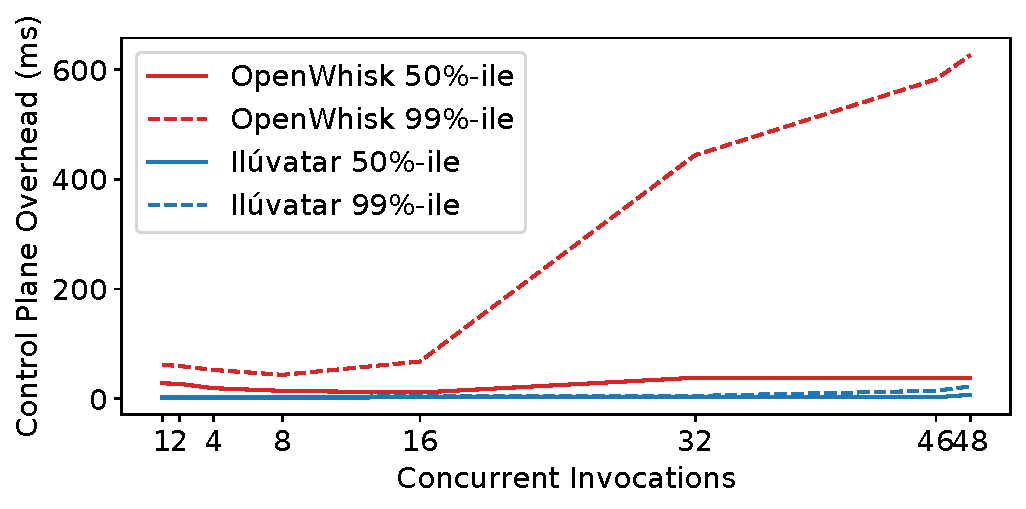
\includegraphics[width=0.4\textwidth]{../graphs/scaling/pyaes/openwhisk-overhead-scaling.pdf}
  \caption{The latency overhead imposed by the control plane, as the number of concurrent invocations increases. Note the log scale. OpenWhisk overhead is significant and has high variance, resulting in high tail latency. Our proposed \sysname can bring this overhead down by more than 100x. }
  \label{fig:ow-scaling}
\end{figure}


\noindent \textbf{Performance.}
%
Because of its central role in coordinating all aspects of function execution, the control plane plays a major role in determining function performance.
Managing the function execution lifecycle for hundreds of concurrent invocations imposes a \emph{control plane overhead}, and increases the end-to-end latency.
This control plane overhead can be significant, and affects \emph{all} function invocations, including and especially the ``warm'' ones. 
This control plane overhead can be measured by subtracting the execution time of the function code from the end-to-end latency.
This overhead for the PyAES function from functionbench~\cite{} is shown in Figure~\ref{fig:ow-scaling}. 

The figure shows the 50 and 99 percentile overheads as the number of concurrent invocations are increased.
In each case, we are invoking the function repeatedly in a closed-loop, and concurrent invocations are obtained by using multiple client threads. All invocations are warm starts.  
The experiment is run on a 48 core server (more details in~\ref{sec:eval}), and the figure shows the performance at low and medium load conditions. 

From Figure~\ref{fig:ow-scaling}, we can see that the OpenWhisk latency overhead is more than 10ms,  which is already a significant increase in latency for small functions which dominate real-world FaaS workloads.
Worryingly, the 99 percentile overhead is much higher, and rises to as much as 600ms.
We also see strange inversions in the scaling behavior: the overhead reduces for certain load-levels, and then increases again.
This high overhead, high variance, and uncertain scaling behavior, results in many challenges for FaaS \emph{providers}. 
Due to these issues, low-latency functions see severe performance degradation, and resource provisioning and capacity planning becomes harder due to the high variance and performance unpredictability.
For the sake of comparison, the figure also shows the latency overhead of \sysname in the same environment.
We are able to achieve a per-invocation mean overhead of less than 2ms for almost all the load conditions.
Importantly, the tail overhead is also small: less than 3ms for less than 32 concurrent invocations, rising to 10ms when the system is saturated. 


To emphasize, for a median function in the Azure workload which runs for X ms, OpenWhisk increases its latency by 50\%. 
Thus, the control plane plays a crucial role in function performance.
We note that these are the best-case warm-start latencies, when the function's containers is fully initialized and in memory. 
Since function cold starts impose such a major performance penalty (increasing latency by more than $10\times$), mitigating them has been a major research focus. 
However, because of temporal and spatial locality of access, caching and prefetching techniques can be extremely effective, and the cold start rate is often less than $1\% $ of all invocations. 
The majority of invocations are thus ``warm'', where the performance is dominated by control plane overheads.
\emph{We thus need a low-latency, low-jitter control plane.}

\textbf{Could do a simple simulation of cplane overhead vs. fn running times.}

\begin{comment}
function performance is impacted more by control plane overheads. 

Because of the non-trivial coordination between various system components (such a


Since function cold starts impose such a major performance penalty (increasing latency by more than $10\times$), mitigating them has been a major research focus.
%Cold starts are a fundamental result of the programming model and isolation requirements.
However, they are 

% Why not focus on cold starts 
Rightly, the large cold start overheads have received a lot of attention with many powerful techniques proposed.
Cold starts are generally rare, especially with a combination of keep-alive and prefetching.
However, the control-plane overhead affects all invocations, including the ``warm starts''.

Large amount of prior work on new containerization techniques for lightweight sandboxing, or reducing cold start overheads via snapshotting etc. 
%
In all this the one component overlooked is the control plane, all the above performance optimizations are complementary to it.
%

Current cplanes are too large and slow. \textbf{Figure here.}
\end{comment}

\noindent \textbf{System Design.}
%
As evidenced by the OpenWhisk architecture presented earlier, FaaS control planes are large, complex distributed systems.
Due to the continually evolving needs of FaaS applications and emergence of new sandboxing techniques (such as lightweight VMs like Firecracker), they are sandwiched between the scale and heterogeneity of FaaS workloads one hand, and the deep stack of OS and virtualization components on the other. 

For instance, systems for running web services or microservices such as~\cite{} do not have to deal with large and highly variable sandbox management overheads, nor with highly heterogeneous request sizes.
For reducing tail latency, these systems can often rely on the OS CPU scheduler for processor sharing, can do CPU allocation at very fine granularity~\cite{}, use queuing theory techniques, etc. 
At the other extreme, for longer running containers and VMs, their control planes, like OpenStack or Kubernetes face a much lower rate of VM arrivals and departures. and can do careful and ``hard'' resource allocation using bin-packing.


Functions are highly heterogeneous, and can be seen as both latency-sensitive web requests \emph{and} large containers requiring significant system resources for several seconds. 
FaaS control planes thus have to do \emph{both} low-latency allocation \emph{and} pack CPU and memory resources on their servers carefully to maintain high system utilization.
%
We posit that these competing needs present new challenges in large-scale distributed resource allocation.
A clean-slate control plane design helps us investigate the fundamental performance tradeoffs and challenges in this fast-evolving ecosystem.
Our new implementation also helps to identify the current performance bottlenecks and new avenues of OS optimizations. 




\begin{comment}
Because of the non-trivial coordination between various system components (such a


Another key challenge is the heterogeneous nature of function workloads. 
Many small functions, and so systems from microservices and ultra-low-latency techniques for CPU scheduling can be applied.
But FaaS servers run mixed workloads and some functions are ``heavy'' can run for several seconds. 
Thus, this is closer to a ``bin packing'' or long-task scheduling problem like with VMs or long-lived containers, where adequate resources must be reserved before launching a task.
Thus there are tradeoffs in the hard vs. soft allocation and the competing demands on performance. 


Finally, the interaction with the containerization and sandboxing layer means that the control plane is decoupled from these lower level layers that are involved in running the functions.
The control plane thus doesnt have direct control over the exact task placement and other techniques that are used for microservices.
There is a lot more asyncrhony involved and multiple levels of the system boundary must be crossed. 

Owhisk has become a major impediment to fast and reliable resource management, and we want to rectify that.
FaaS is still new and not ossified, so still an opportune time for developing new software frameworks.


We were motivated to investigate a clean-slate design and implementation of a FaaS control plane with the necessary capabilities: low-overhead, low-jitter, extensible.
This was approached in an integrated modular fashion by making use of container runtimes, and then building aother components on top of it. 

Thus as part of the clean-slate design, we want to know what are the key design choices and their performance tradeoffs, in order to enhance our understanding of function performance in various scenarios.


\textbf{Table?} OWhisk, Knative, faasd, openfaas, ...
\end{comment}


\noindent \textbf{Platform for Experimental Systems Research.}
%
Performance-focused FaaS research is already challenging due to the extreme scale and heterogeneity of the workloads.
These challenges are compounded by existing control planes like OpenWhisk that are unfortunately highly unpredictable.
The control plane jitter and the extreme bimodal cold vs. warm latencies makes it difficult to do reliable and reproducible research~\cite{mytkowicz2009producing}, and subtle environmental and configuration effects can mask the true effects of new research optimizations. 
With OpenWhisk, function performance can be severely affected by a myriad of configuration options, such as insufficient memory for CouchDB, networking configuration, Docker configuration, etc. 

Given the importance of the control plane, we want \emph{predictable} performance to a large degree. 
In our experience, research in FaaS stymied by the large overheads and complexity of existing control planes.
Thus \sysname is designed from the ground-up to be lightweight and provide predictable performance under different conditions. 
Our system implementation can potentially accelerate the development of new optimizations, clarify  our undestanding of performance characteristics of this relatively new stack, and provide a platform for robust experiments. 



\begin{comment}
\textbf{Why write from scratch instead of improving existing ones?}

A clean-slate design also gives us the opportunity for understanding the design tradeoffs that could be helpful for general FaaS research and 

Lightweight/minimal ones like faasd exist. But again, written in go, not performance focused, and implementing all the desired research features would make it a different.

We also wanted this to be a design exercise in exploring the tradeoff between being lightweight and high performance vs. being extensible and ``full-featured''.
\end{comment}


%%% Local Variables:
%%% mode: latex
%%% TeX-master: "paper"
%%% End:
